\PassOptionsToPackage{dvipsnames}{xcolor}
\documentclass{beamer}
\usepackage{xcolor}
\usepackage{pgfpages}

\usepackage[style=authortitle]{biblatex}

\setbeameroption{show notes on second screen}

\usepackage[utf8]{inputenc}
\usepackage[T1]{fontenc}
\usepackage{lmodern}
\usepackage{fontawesome}

\usepackage{minted}

\usepackage{listings}

\usepackage[american]{babel}

\usepackage{
    amsmath,
    amsfonts,
    amssymb
}

\usepackage[os=win]{menukeys}

\usetheme{UOS}

\graphicspath{{img/}}

% use this with \begin{pythoncode} ... \end{pythoncode}
\newminted{python}{linenos=false}

\newminted[outputcode]{text}{linenos=false}

% this gets rid of red boxes around syntax errors in minted
\AtBeginEnvironment{minted}{%
  \renewcommand{\fcolorbox}[4][]{#4}}

% removes the prefix "Figure 1:" in figure captions
\setbeamertemplate{caption}{\raggedright\insertcaption\par}


\begin{document}

\title[Good Practices]{Week 7: Debugging and Good Practices}
\subtitle{Basic Programming in Python}

\author[kgross, mpoemsl, sselbach]{Katharina Groß, Martin Pömsl, Sören Selbach}

\date{\today}

\begin{frame}[plain]
     \titlepage
\end{frame}

\begin{frame}
    \tableofcontents
\end{frame}

\section{Recap}

\subsection{Working With Files}

\begin{frame}[fragile]{Opening Files}

    \begin{block}{}
        Files need to be \textbf{opened} and \textbf{closed}
    \end{block}

    \vspace{1em}

    \begin{pythoncode}
    my_file = open("some_file.txt")

    contents = my_file.read()
    print(contents)

    my_file.close()
    \end{pythoncode}

\end{frame}

\begin{frame}[fragile]{Opening Files}

    \begin{block}{}
        To make this more convenient, we can use a \textbf{context manager}
    \end{block}

    \vspace{1em}

    \begin{pythoncode}
    with open("some_file.txt") as my_file:
        # my_file is available in this block
        contents = my_file.read()
        print(contents)

    # my_file is closed automatically afterwards
    \end{pythoncode}

    \note{
        There pretty much never is a reason not to use a context manager.
    }

\end{frame}

\begin{frame}{Reading, Writing, Appending}
    By default, files are opened for \textbf{reading} \\
    We need to specify a \textbf{file mode} if we want to write to a file \\
    \vspace{1em}
    \begin{itemize}
        \item \texttt{r}: reading only (default)
        \item \texttt{w}: writing only, overwrites existing content
        \item \texttt{a}: writing only, appends to the end of the files
    \end{itemize}
    \vspace{1em}
    You can add a "\texttt{+}" to make it read and write at the same time
\end{frame}

\subsection{CSV Files}

\begin{frame}[fragile]{CSV Files}

    CSV (\textbf{C}omma \textbf{S}eparated \textbf{V}alue) files are text files with a certain format

    \vspace{1em}

    \begin{exampleblock}{\texttt{names.csv}}
        \begin{outputcode}
    id,last_name,first_name,age
    0,Skywalker,Luke,42
    1,Solo,Han,52
        \end{outputcode}
    \end{exampleblock}

    The first line is a \textbf{header}, the rest contain \textbf{values}

    \vspace{1em}

    Python provides a module for conveniently working with csv files

    \note{
        \begin{itemize}
            \item The \textbf{header} tells you what the values in a certain column mean
            \item CSV files \textbf{may} have a header, but don't have to. Just like they \textbf{may} be separated by commas, but it could also be semicolons. Always have a look at the contents of the files you are working with!
            \item We \textit{could} simply read a csv file like a text file and do the splitting at commas and line breaks by ourselves, but using the \texttt{csv} module is simpler.
        \end{itemize}
    }

\end{frame}

\begin{frame}[fragile]{Using the \texttt{csv} Module}

    \begin{pythoncode}
    import csv

    with open("names.csv") as csv_file:
        reader = csv.reader(csv_file)

        for row in reader:
            print(row)
    \end{pythoncode}

    \textbf{Output:}

    \begin{outputcode}
    ["id", "last_name", "first_name", "age"]
    ["0", "Skywalker", "Luke", "42"]
    ["1", "Solo", "Han", "52"]
    \end{outputcode}

    \note{
        Note that with this approach, you manually have to deal with the header.

        \vspace{1em}

        If you're asking yourself "What is this reader thing and why can I iterate over it?", that's a great question to ask! Unfortunately, to really answer this question we would have to go deeper than this course's scope would allow. For now, imagine it sort of like a \textit{list} that contains all the rows of the file - just keep in mind that it is not \textit{really} a list.
    }

\end{frame}

\begin{frame}[fragile]{Using the \texttt{csv} Module}

    \begin{pythoncode}
    import csv

    with open("names.csv") as csv_file:
        dict_reader = csv.DictReader(csv_file)

        for row in dict_reader:
            print(row)
    \end{pythoncode}

    \textbf{Output:}

    \begin{outputcode}
    {"id": 0, "last_name": "Skywalker", ...}
    {"id": 1, "last_name": "Solo", ...}
    \end{outputcode}

    \note{
        Actually, in current versions of Python, the \texttt{DictReader} will yield \texttt{OrderedDict}s, which look slightly different. You can still use them like any normal dictionary, though!
    }

\end{frame}

\subsection{Recap Lecture}

\begin{frame}{Recap Lecture}
    We will have a \textbf{recap lecture}!

    \vspace{1em}
    If you have any specific topics you would like to see revisited, tell me now or write us an email anytime (before the recap lecture)

    \vspace{1em}
    \texttt{kgross@uos.de \\
    mpoemsl@uos.de \\
    sselbach@uos.de}
\end{frame}

\section{Debugging}

\subsection{Understanding Error Messages}

\begin{frame}{Understanding Error Messages}

    \begin{itemize}
        \item Even the most experienced programmers make \textbf{mistakes}
        \item \textbf{Error messages} help you spot where in your code your mistake is and how you can fix it.
        \item However, they require some \textbf{interpretation}!
    \end{itemize}

    \note{
        One of the hard parts of programming is accepting that the computer does \textit{exactly} what it is told to and in 99.9\% of the cases it is \textit{you} who made a mistake.
    }

\end{frame}

\begin{frame}[fragile]{Understanding Error Messages}

    \begin{alertblock}{}
        \begin{outputcode}
      File "my_file.py", line 42
        print("test"))
                     ^
    SyntaxError: invalid syntax
        \end{outputcode}
    \end{alertblock}

    This tells you:

    \begin{itemize}
        \item which \textbf{file} the error occurred in (\texttt{my\_file.py})
        \item which \textbf{line} the error occurred in (line 42)
        \item where \textbf{in} the line the error occurred (the \texttt{\^})
        \item what \textbf{type} of error it was (SyntaxError)
        \item sometimes some additional information ("invalid syntax")
    \end{itemize}

    \note{
        The caret symbol (\texttt{\^}) is not always as helpful as you may think. For example, there is no way for Python to know \textit{where} you forgot to close a bracket, only \textit{that} you did.
    }

\end{frame}

\begin{frame}{Error Types: \texttt{SyntaxError}}

    A \texttt{SyntaxError} ...

    \begin{itemize}
        \item ... occurs when Python cannot read your code
        \item think of them as grammatical errors
        \item \textbf{Examples:} missing \texttt{)}, missing \texttt{:} etc.
        \item a subtype is the \texttt{IndentationError}
    \end{itemize}

    You can fix them most of the time by reading through the indicated line very carefully.

\end{frame}

\begin{frame}{Error Types: \texttt{NameError}}

    A \texttt{NameError} ...

    \begin{itemize}
        \item ... occurs when a name (e.g. of a variable or function) is referenced that does not exist
        \item they happen for example when
        \begin{itemize}
            \item you misspelled a variable name
            \item you call a function before it is defined
            \item you forgot to import a module
            \item you define a variable in a function (local scope) and try to access it from outside the function
        \end{itemize}
    \end{itemize}

\end{frame}

\begin{frame}{Error Types: \texttt{IndexError} \& \texttt{KeyError}}

    An \texttt{IndexError} ...
    \begin{itemize}
        \item ... occurs when you try to access an element \textbf{by index} that does not exist
        \item \textbf{Example:} You try to access \texttt{my\_list[4]} when \texttt{my\_list} has only 4 elements
    \end{itemize}

    \vspace{1em}

    A \texttt{KeyError} ...
    \begin{itemize}
        \item ... is the same, but for dictionaries, which are accessed \textbf{by key}
        \item \textbf{Example:} You try to access \texttt{my\_dict["c"]} when \texttt{my\_dict} is \texttt{\{"a": 1, "b": 42\}}
    \end{itemize}

    \note{
        \begin{itemize}
            \item note that if \texttt{my\_list} has 4 elements, the last one is \texttt{my\_list[3]} because of indices start at 0!
        \end{itemize}
    }

\end{frame}

\begin{frame}{Error Types: \texttt{TypeError}}

    A \texttt{TypeError} ...
    \begin{itemize}
        \item ... occurs when you try to perform an operation on something of the wrong type
        \item \textbf{Examples:}
        \begin{itemize}
            \item \texttt{"The answer is: " + 42}
            \item \texttt{my\_variable(42)} when \texttt{my\_variable} is not a function
            \item you call a function with a wrong \textbf{number of arguments}
        \end{itemize}
    \end{itemize}

    \vspace{1em}

    TypeErrors can be a bit more tricky to fix

\end{frame}

\begin{frame}{Error Types: \texttt{ValueError}}

    A \texttt{ValueError} ...
    \begin{itemize}
        \item ... occurs when the type of your variable is the correct one for the operation, but the actual value is invalid
        \item \textbf{Examples:}
        \begin{itemize}
            \item \texttt{float("bananas")}
            \item wrong number of elements in a tuple when unpacking
        \end{itemize}
    \end{itemize}

    \note{
        As always, we have only covered some of the more important error messages. Check the docs for more!

        \vspace{1em}

        https://docs.python.org/3/library/exceptions.html\#concrete-exceptions
    }

\end{frame}

\begin{frame}[fragile]{Error Spotting: The Good...}

    \begin{pythoncode}
    word_list   = ["a", "b", "a"]
    trans_dict  = {"a": "X", "b": "Y"}
    translated  = []

    for word in word_list
        translated.append(trans_dict(word))

    print(translated)
    \end{pythoncode}

    \pause
    \textbf{Output:}

    \begin{outputcode}
      File "debug_test.py", line 5
        for word in word_list
                            ^
    SyntaxError: invalid syntax
    \end{outputcode}

\end{frame}

\begin{frame}[fragile]{Error Spotting: The Good ...}

    \begin{pythoncode}
    word_list   = ["a", "b", "a"]
    trans_dict  = {"a": "X", "b": "Y"}
    translated  = []

    for word in word_list:
        translated.append(trans_dict(word))

    print(translated)
    \end{pythoncode}

    \note{
        This one was simple: We forgot a colon \texttt{:} at the end of the \texttt{for}-loop head.
    }

\end{frame}

\begin{frame}[fragile]{Error Spotting: The Good ...}

    \textbf{Output:}

    \begin{outputcode}
    Traceback (most recent call last):
      File "debug_test.py", line 6, in <module>
        translated.append(trans_dict(word))
    TypeError: 'dict' object is not callable
    \end{outputcode}

    \vspace{1em}

    What is the error?
    \begin{itemize}
        \item something in \textbf{line 6}
        \item something involving a \textbf{dictionary}
        \item something about trying to \textbf{call} it
    \end{itemize}

    \pause
    \vspace{1em}

    \textbf{Solution:} We used \texttt{()} (which is used for calling something) instead of \texttt{[]}

    \note{
        This one was already a bit trickier. You needed to figure out where you were trying to call a dict, which requires some more understanding of Python.

        \vspace{1em}

        Did you notice, however, that for fixing both the \texttt{SyntaxError} and the \texttt{TypeError} you did not really need to understand the code? That is why these are "good" errors - they are easy to fix.
    }

\end{frame}

\begin{frame}[fragile]{Error Spotting: The Good ...}

    \textbf{The fixed code:}

    \begin{pythoncode}
    word_list   = ["a", "b", "a"]
    trans_dict  = {"a": "X", "b": "Y"}
    translated  = []

    for word in word_list:
        translated.append(trans_dict[word]))

    print(translated)
    \end{pythoncode}

    \textbf{Output:}

    \begin{outputcode}
    ['X', 'Y', 'X']
    \end{outputcode}

\end{frame}


\begin{frame}[fragile]{Error Spotting: ... the Bad ...}

    \begin{pythoncode}
user_input = input("Enter a number: ")

# split to remove whitespaces
user_input = user_input.split()

print(float(user_input))
    \end{pythoncode}

    \pause
    \textbf{Output:}

    \begin{outputcode}
Traceback (most recent call last):
  File "debug_test.py", line 6, in <module>
    print(float(user_input))
TypeError: float() argument must be a string or a number,
not 'list'
    \end{outputcode}

\end{frame}

\begin{frame}[fragile]{Error Spotting: ... the Bad ...}

    \begin{outputcode}
Traceback (most recent call last):
  File "debug_test.py", line 6, in <module>
    print(float(user_input))
TypeError: float() argument must be a string or a number,
not 'list'
    \end{outputcode}

    \vspace{1em}

    \begin{block}{Problem}
        The actual error is nowhere near the indicated line!
    \end{block}

    \note{
        This error is yet a bit more difficult to solve. We need to figure out \textbf{why} \texttt{user\_input} does not have the type we expect, which requires tracing back where it comes from, what changes are made to it etc.
    }

\end{frame}

\begin{frame}[fragile]{Error Spotting: ... the Bad ...}

    \textbf{The fixed code:}

    \begin{pythoncode}
user_input = input("Enter a number: ")  # string

# split to remove whitespaces
user_input = user_input.split()         # list
user_input = "".join(user_input)        # string

print(float(user_input))
    \end{pythoncode}

\end{frame}

\begin{frame}[fragile]{Tracebacks}

    \begin{block}{}
        Very often, errors happen inside a function call
    \end{block}

    In that case, you get a \textbf{traceback}:

    \vspace{1em}

    \begin{outputcode}
Traceback (most recent call last):
  File "debug_test.py", line 7, in <module>
    outer_function()
  File "debug_test.py", line 2, in outer_function
    inner_function()
  File "debug_test.py", line 5, in inner_function
    print("2" + 2)
TypeError: can only concatenate str (not "int") to str
    \end{outputcode}

    \note{
        A traceback is a list of all the function calls that led to the error:
        \begin{itemize}
            \item the last entry in the list is \textbf{the actual line} that produced the error
            \item the entry before that is the line that \textbf{called the function} that produced the error
            \item the entry before that is the line that \textbf{called the function that called the function} that produced the error, a.s.o.
        \end{itemize}

        \vspace{1em}

        This can be very helpful in more complicated programs, where there are many nested function calls distributed over many different files
    }

\end{frame}

\subsection{Logical Errors}

\begin{frame}[fragile]{Error Spotting: ... and the Ugly}

    There is an entirely different kind of error: The one that \textbf{does not produce an error message}

    \vspace{1em}

    \begin{block}{Task}
        We have a list of lines of text and want to delete all empty lines
    \end{block}

    \begin{pythoncode}
    def delete_empty_lines(lines):
        for line in lines:
            if line == "":
                # if empty, remove line
                lines.remove(line)
    \end{pythoncode}

    \note{
        These errors are usually the ones that are the hardest to fix, because you have no error message that tells you where it happens - it could be anywhere in your code! Usually, there is a lot of guessing involved.
    }

\end{frame}

\begin{frame}[fragile]{Error Spotting: ... and the Ugly}

    \begin{pythoncode}
    # in this case it works
    lines_1 = ["blah", "", "blah"]
    delete_empty_lines(lines_1)
    print(lines_1)  # ["blah", "blah"]

    # in this case it does not work!
    lines_2 = ["blah", "", "", "blah"]
    delete_empty_lines(lines_2)
    print(lines_2)  # ["blah", "", "blah"]
    \end{pythoncode}

    \vspace{1em}

    \textbf{What is happening here?}

\end{frame}

\begin{frame}[fragile]{Error Spotting: ... and the Ugly}

    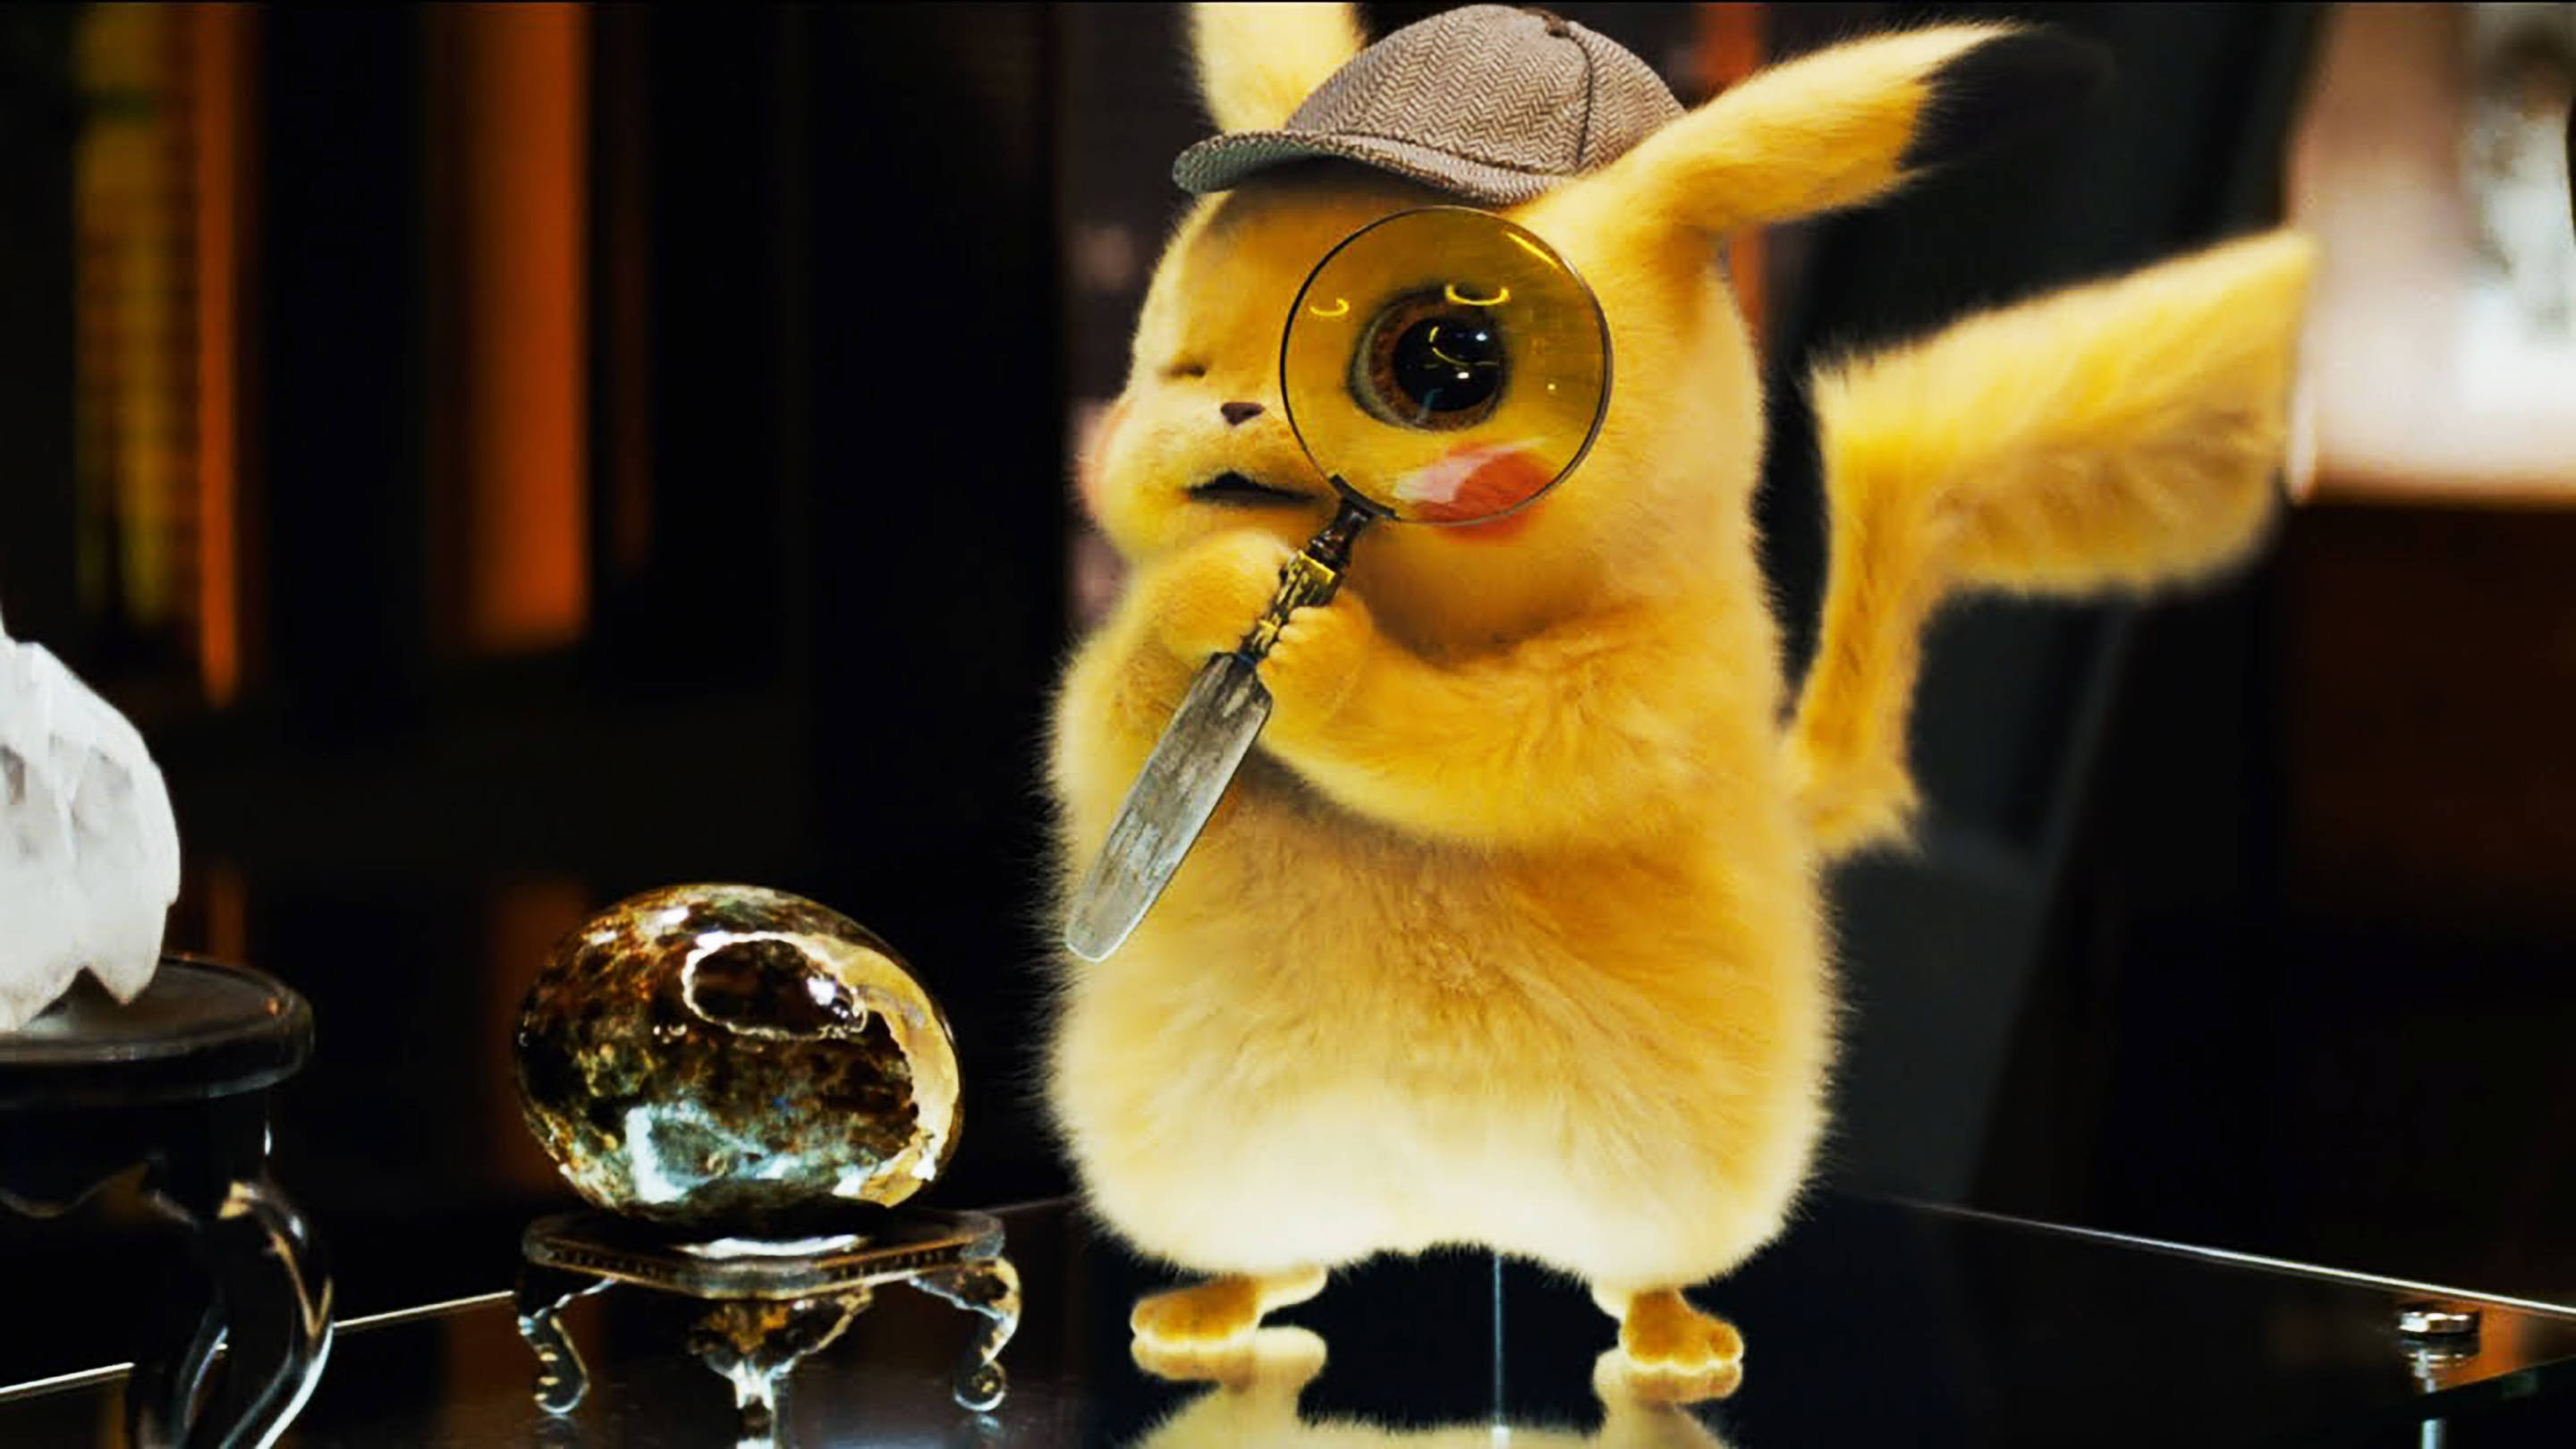
\includegraphics[width=\textwidth]{07_Good_Practises/detective-pikachu.jpg}

    \note{
        https://d11nuriyhamvfv.cloudfront.net/uploads/media/2019/02/27/detective-pikachu\_16x9.jpg
    }

\end{frame}

\begin{frame}[fragile]{Error Spotting: ... and the Ugly}

    We can try out \textbf{different input values}:

    \begin{pythoncode}
    lines_3 = ["blah", "", "", "", "blah"]
    delete_empty_lines(lines_3)
    print(lines_3)  # ["blah", "", "blah"]
    # same result as with lines_2

    lines_4 = ["blah", "", "", "", "", "blah"]
    delete_empty_lines(lines_4)
    print(lines_4)  # ["blah", "", "", "blah"]
    # different result!
    \end{pythoncode}

    \vspace{0.5em}

    \begin{alertblock}{\textbf{Conclusion}}
        Every second consecutive empty line seems to be ignored
    \end{alertblock}

    \note{
        Sometimes, it is enough to play with the inputs a bit to understand what the problem is. \\
        Not in this case, though. We need an even deeper understanding of what is going on.
    }

\end{frame}

\begin{frame}[fragile]{Error Spotting: ... and the Ugly}

    We can \textbf{print intermediate results}:

    \begin{pythoncode}
    def delete_empty_lines(lines):
        for line in lines:
            # print before every iteration
            print("debug:", lines, line)

            if line == "":
                lines.remove(line)
    \end{pythoncode}

    \vspace{1em}

    ... and hopefully find where it goes wrong

    \note{
        The next approach is to print \textbf{intermediate results} to the console in every iteration. This way, we can hopefully see exactly at what point the error occurs. Here, we print both the current value of \texttt{line} and the entire list we are working on, because those are the critical variables that are changing during the loop.

        \vspace{1em}

        A more sophisticated version of this is called logging: This is where you dump a lot of runtime information to a separate file, called a \textit{log file}.

        \vspace{1em}

        When using simple \texttt{print}-statements like this, make sure to remove them when the bug is fixed - or your lecturers might get annoyed ;)
    }

\end{frame}

\begin{frame}[fragile]{Error Spotting: ... and the Ugly}

    We can \textbf{print intermediate results}:

    \begin{pythoncode}
    lines_2 = ["blah", "", "", "blah"]
    delete_empty_lines(lines_2)
    print(lines_2)
    \end{pythoncode}

    \textbf{Output:}

    \begin{outputcode}
    debug: ['blah', '', '', 'blah'] blah
    debug: ['blah', '', '', 'blah']
    debug: ['blah', '', 'blah'] blah
    ['blah', '', 'blah']
    \end{outputcode}

    \note{
        And there we have our bug! Let's go through the steps:
        \begin{enumerate}
            \item the first item is \texttt{"blah"}, which is not an empty line, and so we just move on
            \item the second item is \texttt{""}, which \textbf{is} an empty line, and so we remove it from the list. Note that the list now looks like this: \texttt{["blah", "", "blah"]}
            \item because last, we looked at the second item, by definition of iteration we now look at the third item. \textbf{But the third item has changed} because we removed one before it! And thus, we skipped over element, which happened to be an empty line.
        \end{enumerate}

        The problem ultimately boils down to the fact that we \textbf{modified a list} (not just individual elements) \textbf{while iterating over it!}
    }

\end{frame}

\begin{frame}[fragile]{Error Spotting: ... and the Ugly}

    \begin{block}{\textbf{Solution}}
        We create a new list where we only append lines that are not empty
    \end{block}

    \textbf{The fixed Code:}

    \begin{pythoncode}
    def delete_empty_lines(lines):
        filtered = []

        for line in lines:
            if line != "":
                filtered.append(line)

        return filtered
    \end{pythoncode}

    \note{
        This works because we leave the original list untouched while we iterate over it. Note that it differs slightly in application, as we do not modify the original list but instead return a new list.

        \vspace{1em}

        There are many more ways we could have fixed that bug - it is a good exercise to come up with some more!
    }

\end{frame}

\begin{frame}{Debuggers}
    \begin{itemize}
        \item \textbf{Debuggers} are tools that help you find the origin of errors
        \item they allow you to set \textbf{breakpoints} that pause the program and let you inspect the value of variables
        \item they can do many more things that are more or less helpful
        \item they are provided by many IDEs as well as the \texttt{pdb} module
        \item we will not cover them in this course
    \end{itemize}

    \note{
        IDE: \textit{\textbf{I}ntegrated \textbf{D}evelopment \textbf{E}nvironment}

        \vspace{1em}

        An IDE is a code editor, but also provides many more functionalities like said debuggers or being able to directly run your code on the press of a button. Using IDEs can be helpful if you work on larger projects - but they will not automatically make you a better programmer.
    }
\end{frame}


\subsection{Handling Exceptions}

\begin{frame}[fragile]{Handling Exceptions}

    \begin{block}{}
        Sometimes, you \textbf{expect} your program to fail in a certain spot
    \end{block}

    \begin{pythoncode}
    user_input  = input("Enter a number: ")

    # convert to float
    user_number = float(user_input)
    \end{pythoncode}

    \vspace{1em}

    \begin{itemize}
        \item if the user enters something that cannot be converted to \texttt{float}, a \texttt{ValueError} is raised
        \item we do not want that to crash our program
    \end{itemize}

    \note{
        \textit{Exception} is often used synonymously with \textit{Error}. Exceptions can be more general, however.

        \vspace{1em}

        For instance, when a user presses \keys{\ctrl + C}, a \texttt{KeyboardInterrupt} exception is raised, which will "crash" your program just like any error. However this time, it is expected behavior, because \keys{\ctrl + C} \textit{should} stop a program.
    }

\end{frame}

\begin{frame}[fragile]{Handling Exceptions}

    \begin{block}{}
        Python provides the tools to \textbf{catch} Exceptions and \textbf{handle} them
    \end{block}

    \begin{pythoncode}
    user_input = input("Enter a number: ")

    try:
        # try to convert to float
        user_number = float(user_input)

    except ValueError:
        print("That wasn't a number, dummy.")
    \end{pythoncode}

    \vspace{1em}

    So far, this is just a worse error message

    \note{
        Usage of \texttt{try} is simple:
        \begin{itemize}
            \item \texttt{try} block: Here goes everything that could potentially fail
            \item \texttt{except Exception} line: Here goes the \textbf{type of exception} you expect. It is also possible to leave out the Exception - but you should \textbf{never ever do that}. What if some other error that you did \textbf{not} expect occurs in the \texttt{try} block? It would not show \textbf{any} error message, making it incredibly difficult to track down.
            \item \texttt{except} block: Here goes what should be \textbf{executed} in case of above specified Exception.
            \item There is also a \texttt{finally} and an \texttt{else} block, which we will not cover here. It could be worth checking out if you deal with Exceptions a lot.
        \end{itemize}
    }

\end{frame}

\begin{frame}[fragile]{Usage Example}

    \begin{pythoncode}
user_number = None

while not user_number:
    try:
        user_input  = input("Enter a number: ")
        user_number = float(user_input)

    except ValueError:
        print("That wasn't a number, try again.")

print("Congratulations, you made it!")
    \end{pythoncode}

    \note{
        In this example we use \texttt{try} and \texttt{except} to keep asking the user to input a number until he finally enters a value that can be converted to float.

        \vspace{1em}

        The value \texttt{None} in Python is used to signal that a variable is intended to be empty at this point, e.g. because we do not know the true value yet that it is supposed to have. Remember that it is a \textit{falsy} value, a fact that our example makes use of.

        \vspace{1em}

        Here is a list of all Exceptions that exist in Python. Keep in mind that external libraries may add their own if you use them.

        \vspace{1em}

        \texttt{https://docs.python.org/3.6/library/\\exceptions.html\#exception-hierarchy}

    }

\end{frame}

\begin{frame}[fragile]{Usage Example}

    \textbf{Output:}

    \begin{outputcode}
    Enter a number: blah
    That wasn't a number, try again.
    Enter a number: blub
    That wasn't a number, try again.
    Enter a number: 42
    Congratulations, you made it!
    \end{outputcode}

\end{frame}


\section{Good Practices}

\begin{frame}{Conventions}

    \begin{itemize}
        \item \textbf{conventions} help with code readability \& debugging
        \item there are rules for:
        \begin{itemize}
            \item how to \textit{structure} your code
            \item where to put \textit{spaces} and \textit{empty lines}
            \item how to \textit{name} your variables, functions etc.
            \item many, many more things
        \end{itemize}
        \item there is an official Python style guide: \textbf{PEP-8} \\
            \url{https://www.python.org/dev/peps/pep-0008/}
        \item try to follow conventions, but don't spend more time on it than on actual coding
        \item what is most important: keep your style \textbf{consistent} within a project
    \end{itemize}


    \note{
        Very often when coding we make decisions that do not affect the result of our program, but only the code itself (e.g. what name to give your variable, how to structure your code, put a space here or nah?). Because we do not want that to take a significant amount of brain power, which should instead be used for more important things, there exist conventions.

        \vspace{1em}

        \textbf{Conventions} tell you (often quite exactly) how to format and structure your code, which feature to use if possible and so on. This can be helpful for you, because you don't need to think about that anymore - but it is invaluable to everyone who reads the code (inluding your future self). If your code has comments, it might not take me an hour to understand it but only 10 minutes. There is a famous saying that goes "code is read much more often than it is written".
    }

\end{frame}

\subsection{Code Structure}

\begin{frame}[fragile]{Code Structure Example}

    \begin{pythoncode}
    """Docstring"""
    import module_1
    import module_2

    GLOBAL_CONSTANT = 42

    def function_1():
        # ...

    def main_function():
        # ...

    main_function()
    \end{pythoncode}

    \note{
        Your code structure \textit{could} look like this:
        \begin{enumerate}
            \item a \textbf{docstring} that explaings what your program does
            \item all \textbf{imports} you will need throughout the entire code
            \item \textbf{constants} that will not change over the course of the program (but should still be easily accessible for testing different values)
            \item \textbf{function} definitions that will be used in your main code
            \item the piece of code that strings all the functions together - ideally, this is very short \\
                you could even have a function called \texttt{main} and your only line that is not inside a function is \texttt{main()}
        \end{enumerate}
        However, there may always be reasons to choose a different code structure. Just make sure it is \textbf{consistent} throughout your project.
    }

\end{frame}

\subsection{Comments \& Docstrings}

\begin{frame}{Comments \& Docstrings}
    \textbf{Documenting} your code helps both others and yourself understand what you did

    \begin{itemize}
        \item you should add \textbf{explanatory comments}
        \begin{itemize}
            \item before a line or group of lines that are not entirely obvious
            \item with the same indentation as the code they describe
            \item \textbf{only rarely} in the same line as the code it describes
        \end{itemize}
        \item you should add \textbf{docstrings}
        \begin{itemize}
            \item as the \textbf{first line} of \textbf{every function}
            \item as the \textbf{first line} of your \textbf{module} (i.e. your program)
        \end{itemize}
        \item you should \textbf{not} add comments
        \begin{itemize}
            \item that are \textbf{self-explanatory} (like: \texttt{x = x + 1   \# increment x})
            \item that are plain \textbf{wrong} (this is worse than no comments at all)
        \end{itemize}
    \end{itemize}
\end{frame}

\subsection{Whitespaces}

\begin{frame}{Whitespaces}
    \textbf{Whitespaces} in the right places can greatly increase readability

    \vspace{1em}

    Do put spaces:
    \begin{itemize}
        \item after commas, colons and semicolons
        \item around \texttt{=}, \texttt{+=}, etc. in assignments
        \item around most binary operators, e.g. \texttt{2 + 2}
    \end{itemize}

    Do \textbf{not} put spaces:
    \begin{itemize}
        \item between a function name and \texttt{()}
        \item around \texttt{=} in keyword arguments
        \item after \texttt{(} and before \texttt{)}
    \end{itemize}

    \note{
        There are of course exceptions - for instance, \texttt{x*y + x*y} is fine, even though there are no spaces around \texttt{*}. This is because they are an operator that binds more strongly than \texttt{+} and thus, this increases readability.

        \vspace{1em}

        When in doubt, use your own judgement to decide what is more readable.
    }

\end{frame}

\begin{frame}[fragile]{Whitespaces: Example}

    \begin{pythoncode}
    # Bad:
    def my_function ( a,b,c ) :
        some_dict={"a" : "b", 4:5}
        another_function(a+b+c, n = 42)

    # Good:
    def my_function(a, b, c):
        some_dict = {"a": "b", 4: 5}
        another_function(a + b + c, n=42)
    \end{pythoncode}

\end{frame}

\begin{frame}{Blank Lines}

    \textbf{Blank lines} and \textbf{linebreaks} in the right places can greatly increase readability

    \vspace{1em}

    \begin{itemize}
        \item separate \textbf{function definitions} by two blank lines
        \item separate \textbf{code blocks} (e.g. loops, if-statements) by a blank line
        \item separate \textbf{logical segments} in your code by line breaks \\
            as a rule of thumb: no more than 4 lines without a blank
        \item \textbf{break up} long lines of code into multiple ones
        \begin{itemize}
            \item ... either \textit{logically}, by using intermediate results saved in variables
            \item ... or \textit{syntactically}, by breaking at supported points in the line
        \end{itemize}
    \end{itemize}

    \note{
        Defining an \textbf{intermediate variable}, even though it may not be strictly necessary, can help break up long and complicated lines of code.

        \vspace{1em}

        \textit{Instead of writing this}

        \vspace{1em}

        \texttt{result = f1(f2(x) + f3(y) ** 2, n=42)}

        \vspace{1em}

        \textit{consider writing this}

        \vspace{1em}

        \texttt{intermediate = f2(x) + f3(y) ** 2} \\
        \texttt{result = f1(intermediate, n=42)}
    }

\end{frame}

\begin{frame}[fragile]{How to Break Up Lines}

    \begin{pythoncode}
    # implicit continuation inside ()
    function_with_many_kwargs(
        kwarg_1=42,
        kwarg_2=84,
        kwarg_3=None)

    # explicit continuation
    total_income = gross_income \
                   - taxes \
                   - student_loan_interest
    \end{pythoncode}

    \note{
        Implicit continuation works with all brackets (i.e. \texttt{()}, \texttt{[]} and \texttt{\{\}}), in almost all situations - be it function arguments, a long list definition or some really, really long index.
    }

\end{frame}

\subsection{Naming Conventions}

\begin{frame}{Naming Conventions}

    \textbf{Naming conventions} exist to make it clear what a name refers to

    \vspace{1em}

    \begin{itemize}
        \item variable and function names should be \texttt{lower\_case\_with\_underscores}
        \item constants should be \texttt{UPPER\_CASE\_WITH\_UNDERSCORES}
        \item classes should be \texttt{UpperCamelCase}
        \item finde a balance between descriptiveness and length
        \begin{itemize}
            \item good: \texttt{translation\_dict}, \texttt{word\_counter}
            \item bad: \texttt{a}, \texttt{list\_for\_storing\_all\_the\_words\_of\_the\_text}
        \end{itemize}

    \end{itemize}

    \note{
        \begin{itemize}
            \item of course, there are no \textit{real} constants in Python, only variables - but that makes it all the more important to stick to this naming convention so that no one accidentally changes them
            \item don't worry about what classes \textit{are}, yet - you will hate them soon enough ;)
        \end{itemize}

        \vspace{1em}

        In Python, many things are handled by convention alone that are hard rules in other languages. For instance, there is no such thing as a private variable in Python, all you can do is to start its name with an underscore \_, which tells other modules that might use your code not to touch it.
    }

\end{frame}

\begin{frame}{Naming Conventions}

    \begin{itemize}
        \item Do \textbf{not} use names for your variables that are already in use by Python!
        \begin{itemize}
            \item \textbf{Examples:} \texttt{list}, \texttt{str}, \texttt{int}
            \item code editors often show those names in a different color
            \item ... and usually they are not very descriptive anyways
        \end{itemize}
    \end{itemize}

\end{frame}

\section{Lecture 13}

\begin{frame}{Lecture 13}

    In our last lecture, we want to talk about an application topic of \textbf{your} choice!

    \vspace{1em}

    There will be a Stud.IP poll, as well as an email

    \vspace{1em}

    In all cases we will look at some external library and show you how you can install those using \texttt{conda} or \texttt{pip}

\end{frame}

\begin{frame}{Topic: NumPy and Pandas}

    \textbf{NumPy:}

    \begin{itemize}
        \item pure Python is slow when working with large lists of numbers
        \item NumPy is a framework for working with large numerical arrays
        \item things like Matrix multiplication become easy with NumPy
    \end{itemize}

    \textbf{Pandas:}

    \begin{itemize}
        \item builds on NumPy
        \item provides more sophisticated data structures for data analysis
        \item think of it like very powerful spreadsheets
    \end{itemize}

    \textbf{This is probably the hardest topic of the four}

\end{frame}

\begin{frame}{Topic: Natural Language Processing}

    Natural Language Processing is the field of analyzing human language with computers

    \vspace{1em}

    For Python, there exists the Natural Language Toolkit (\textbf{NLTK}), as well as \textbf{spaCy}

\end{frame}

\begin{frame}{Topic: Psychological Experiments}

    With the \textbf{Expyriment} library, you can create your own time-critical cognitive experiments, like measuring reaction times

\end{frame}

\begin{frame}{Topic: Data Visualization}

    The \textbf{matplotlib} library allows you to easily create your own plots of your data

    \vspace{1em}

    This can also be done by Pandas, but here we would \textbf{only} focus on visualization

\end{frame}


\end{document}
